% LaTeX file for a 1 page document
\documentclass[12pt]{article}
\usepackage{amsmath}
\usepackage{amssymb}
\usepackage{amsthm}
%\usepackage{physymb}
\usepackage{graphicx}
%\usepackage{wrapfig}
\bibliographystyle{plain}
\usepackage{tikz}
\usepackage{natbib}
\usetikzlibrary{calc,patterns,decorations.pathmorphing,decorations.markings}

\title{Simulation of an Orrery in Box2D\\ A CS296 Report by Group 07}
\author{Ranveer Aggarwal (120050020) \\ ranveeraggarwal@gmail.com \\ \\ Devdeep Ray (120050007) \\ devdeep.ray1994@iitb.ac.in\\ \\Sasibhushan Rallabandi (120050056) \\ sasiralla@iitb.ac.in}
\date{}

\begin{document}
\maketitle

\section{Introduction}
An orrery is a mechanical model of the solar system device that illustrates the relative sizes, positions, and motions of the planets and moons according to the heliocentric model.
\\
\\
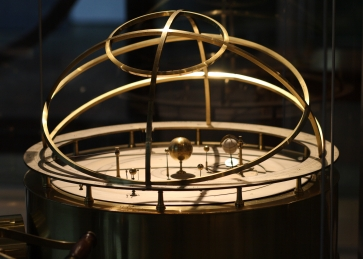
\includegraphics[scale=0.8]{./img/orrery-main.jpg}
\\
Though the Greeks had working planetaria, the first orrery that was a planetarium of the modern era was produced in 1704, and one was presented to the Earl of Orrery — whence came the name. They are typically driven by a clockwork mechanism with a globe representing the Sun at the centre, and with a planet at the end of each of the arms.

\section{The Idea}
\subsection{Initial Design}
Our intial design that we made in Inkscape looked like this:
\\ \\
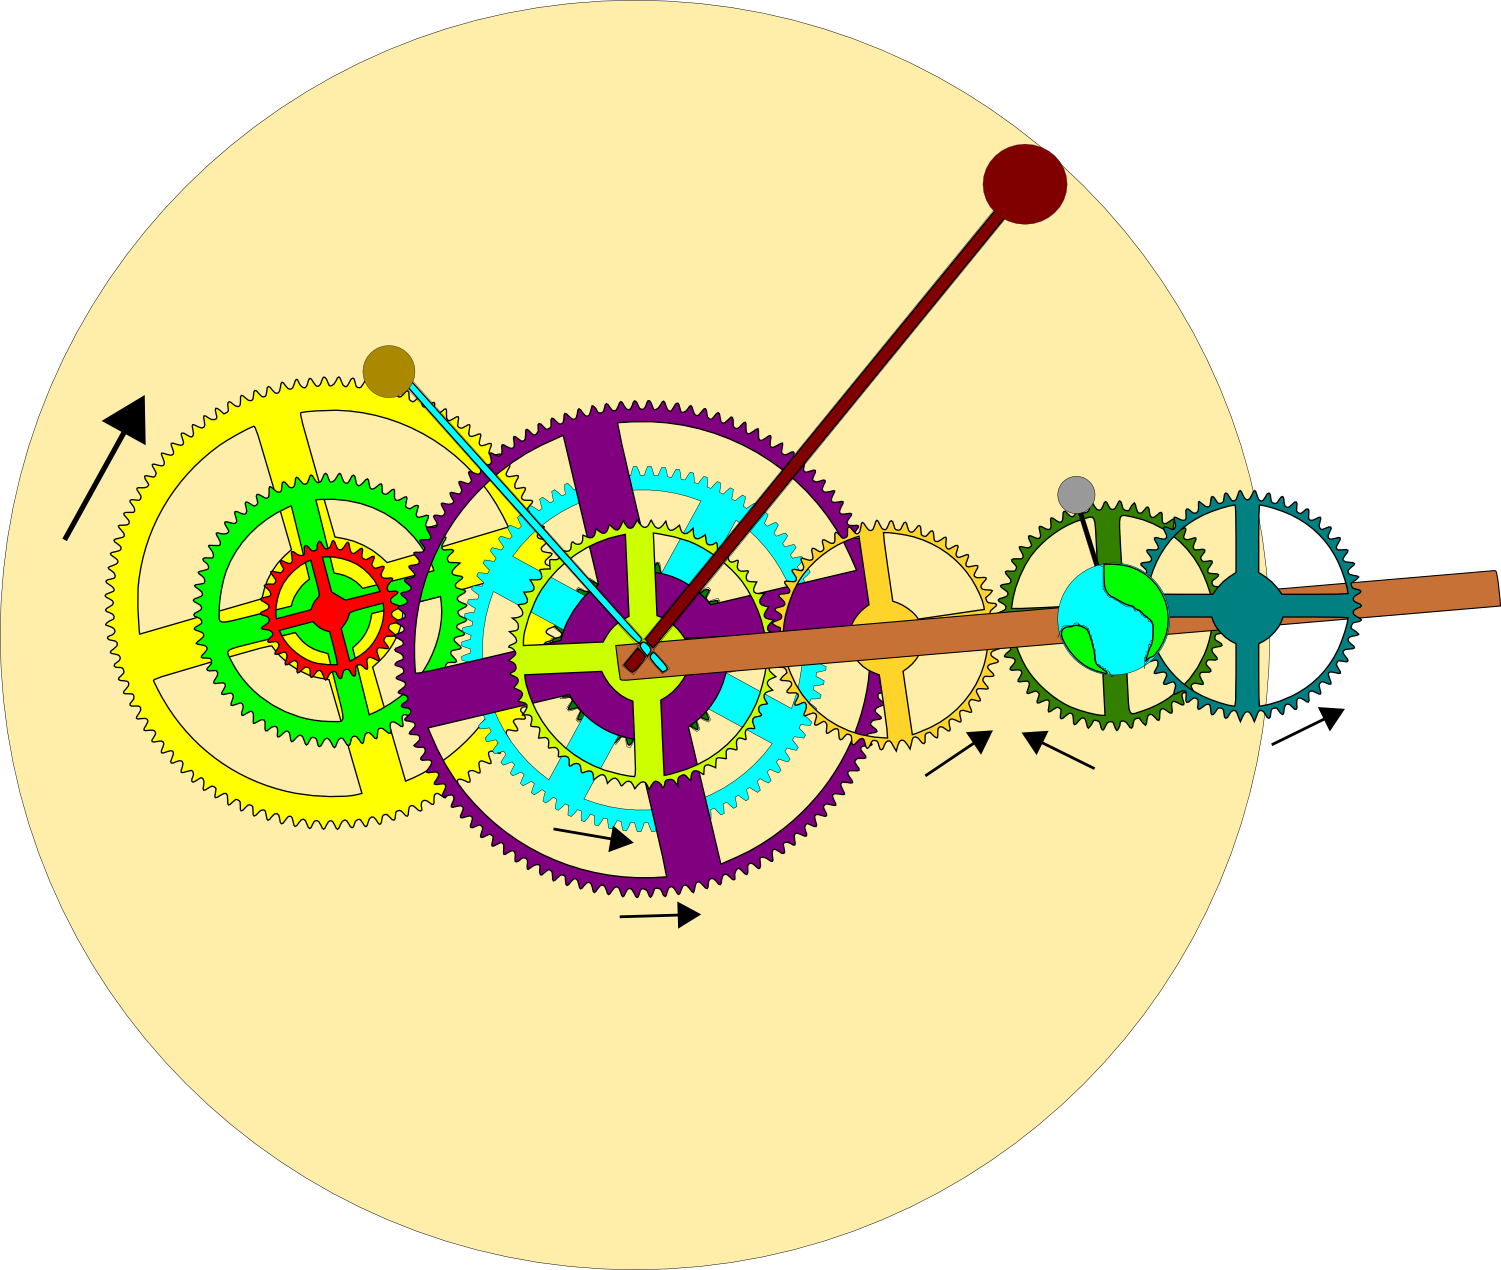
\includegraphics[scale=0.1]{./img/svg.png}
\\

The leftmost gear system is the driving gear system. It is driven by a motor and is coupled to the planet gears to give different speed to each planet. The moon is driven by a chain of gear having different $\omega$ than $\omega_{earth}$. This makes the moon revolve around the earth. In this way, choosing the correct radius values, we can simulate a part of the solar system.

The system simulated through this arrangement assumed perfectly circular orbits, i.e. we neglected that the actual celestial orbits are a bit elliptical. Also, since the scope for error in calculations in Box2D is quite high, the system simulated by us doesn't take the exact ratios of orbits. We just tried to simulate the relative faster/slower speed. For example the Earth revolves slower than Venus and Jupiter slower than the Earth. This has been incorporated in our design.

\subsection{Deviation from the Original Design}
During the course of doing this project, we learnt a lot more than what we knew initially and we discovered what will work and what wont. Hence, we continuously modified our design to reach to the final output, that looks like this:
\\ \\
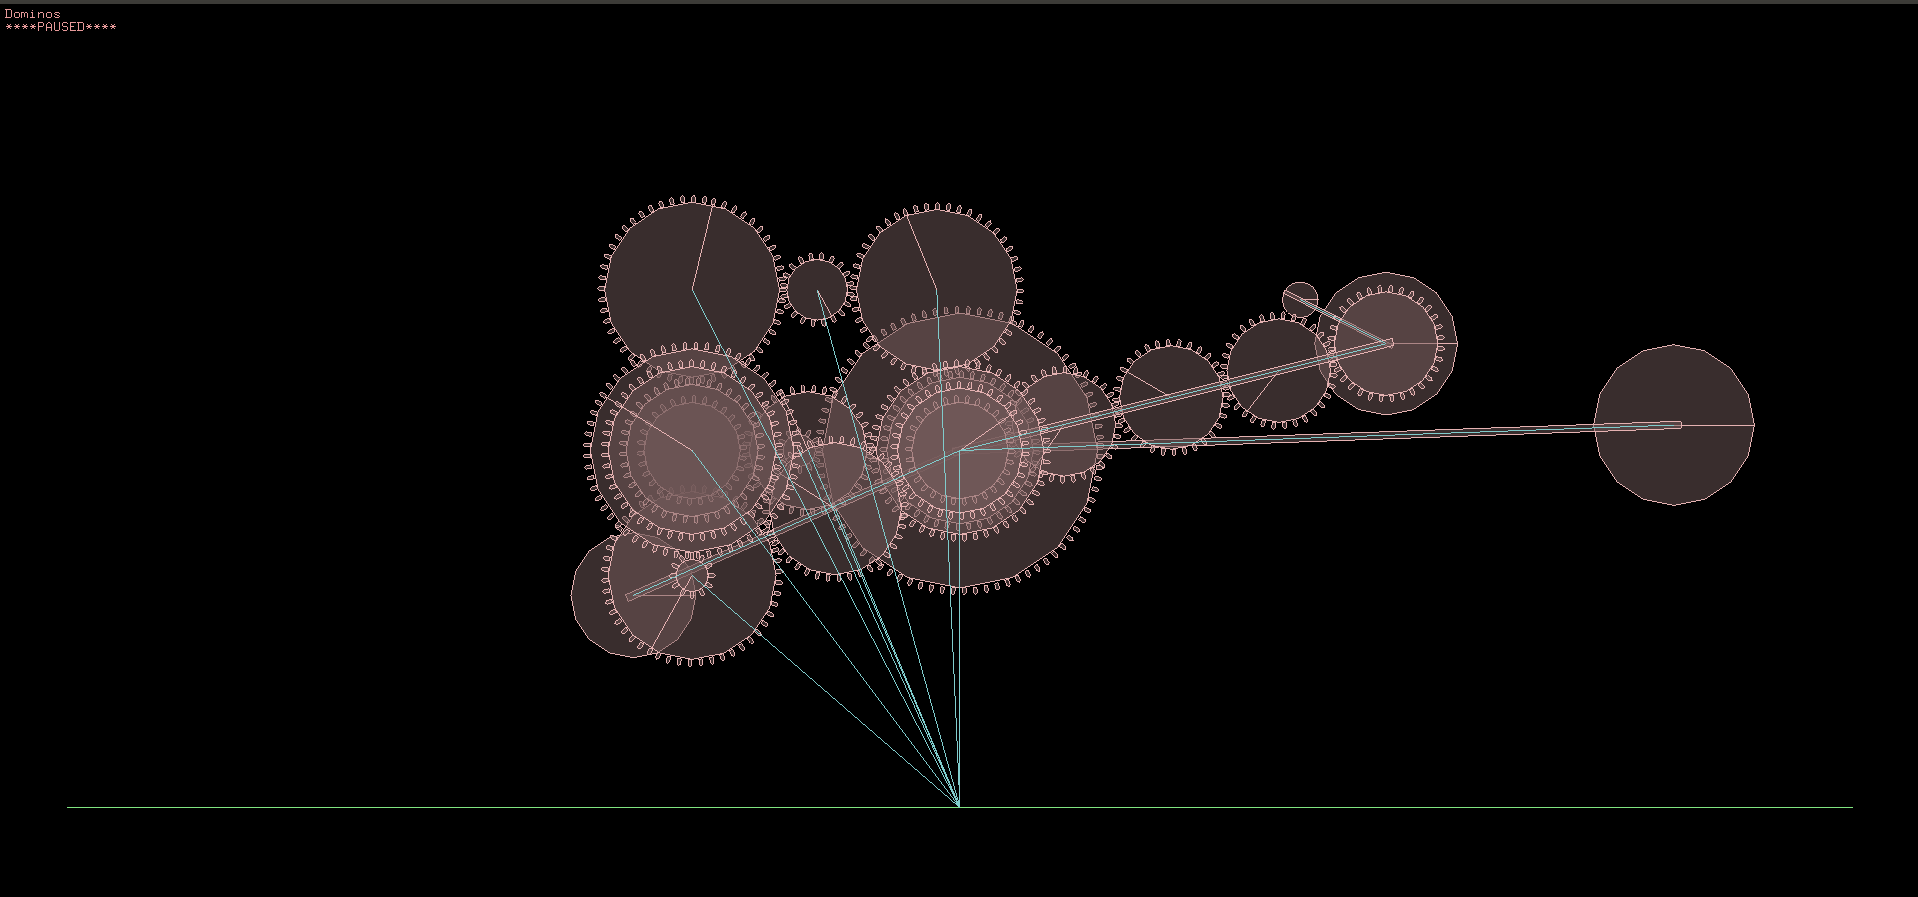
\includegraphics[scale=0.25]{./img/gui.png}
\\

The concept is the same. We planned the gear placements better to make the thing look less cluttered. 

Now, we have a central stack which has all the planet driving gears along with the main driver gear, all of these being disjoint and relatively free to move. Motion from the main driver gear is transferred to the subsequent gears through a series of gears on the sides of the stack as seen from the figure. The driver motion is transferred to mars, whose motion is transferred to Earth, whose motion is transferred to the moon and venus and venus' motion is transferred to mercury.

The mathematics used here is basic geometry and trigonometry to calculate the gear positions and the gear radii so that they are in precise contact.

\section{Points of Interest}
Simulating a natural phenomenon via a mechanical simulation is in fact pretty intersting. Whereas the actual solar system works on gravitational pull between celestial bodies, this system is purely contact driven. 

While on first look it looks pretty elementary -- one could have a series of motors attached to rods to rotate the bodies as needed, but here, what we have done is, we have controlled the whole system through just one motor, i.e., changing one small motor parameter influences the whole system.

This has been done by calculating ratios of gear radii and also, the number of gears from the driver gear to the body.

Again, to make things simpler, one could have just used gear joints to connect circles and run the whole system smoothly without any sort of complication. But, we chose to make our own gear and instead of using gear joints, we relied on contact forces like friction to drive our system.

Here is how our gear looks like:
\\ \\
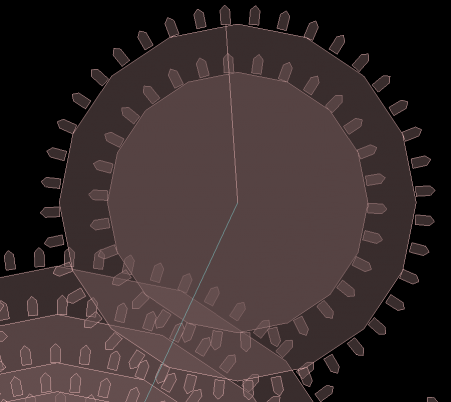
\includegraphics[scale=0.4]{./img/gear.png}
\\
As you can see, we have a circle and on it, a series of polygons (pentagons, can be made into sqares by uncommenting a part) that collide with each other to transfer motion. Since the pivot of the gear gives no anti-torque (frictionless), we guarantee that the gears do not stop. 

Our early design had triangles as teeth. That didn't work out as the teeth kept slipping off -- the design wasn't robust. Then we switched over to squares. It had a completely opposite problem -- the teeth stuck to each other when their sides touch. So, we combined both of these and came up with the pentagon which worked pretty well.
\pagebreak
\section{Code Analysis}
\subsection{Analysis with gprof Using a Callgraph}
Here's the callgraph we got running the debug profile:
\\ \\
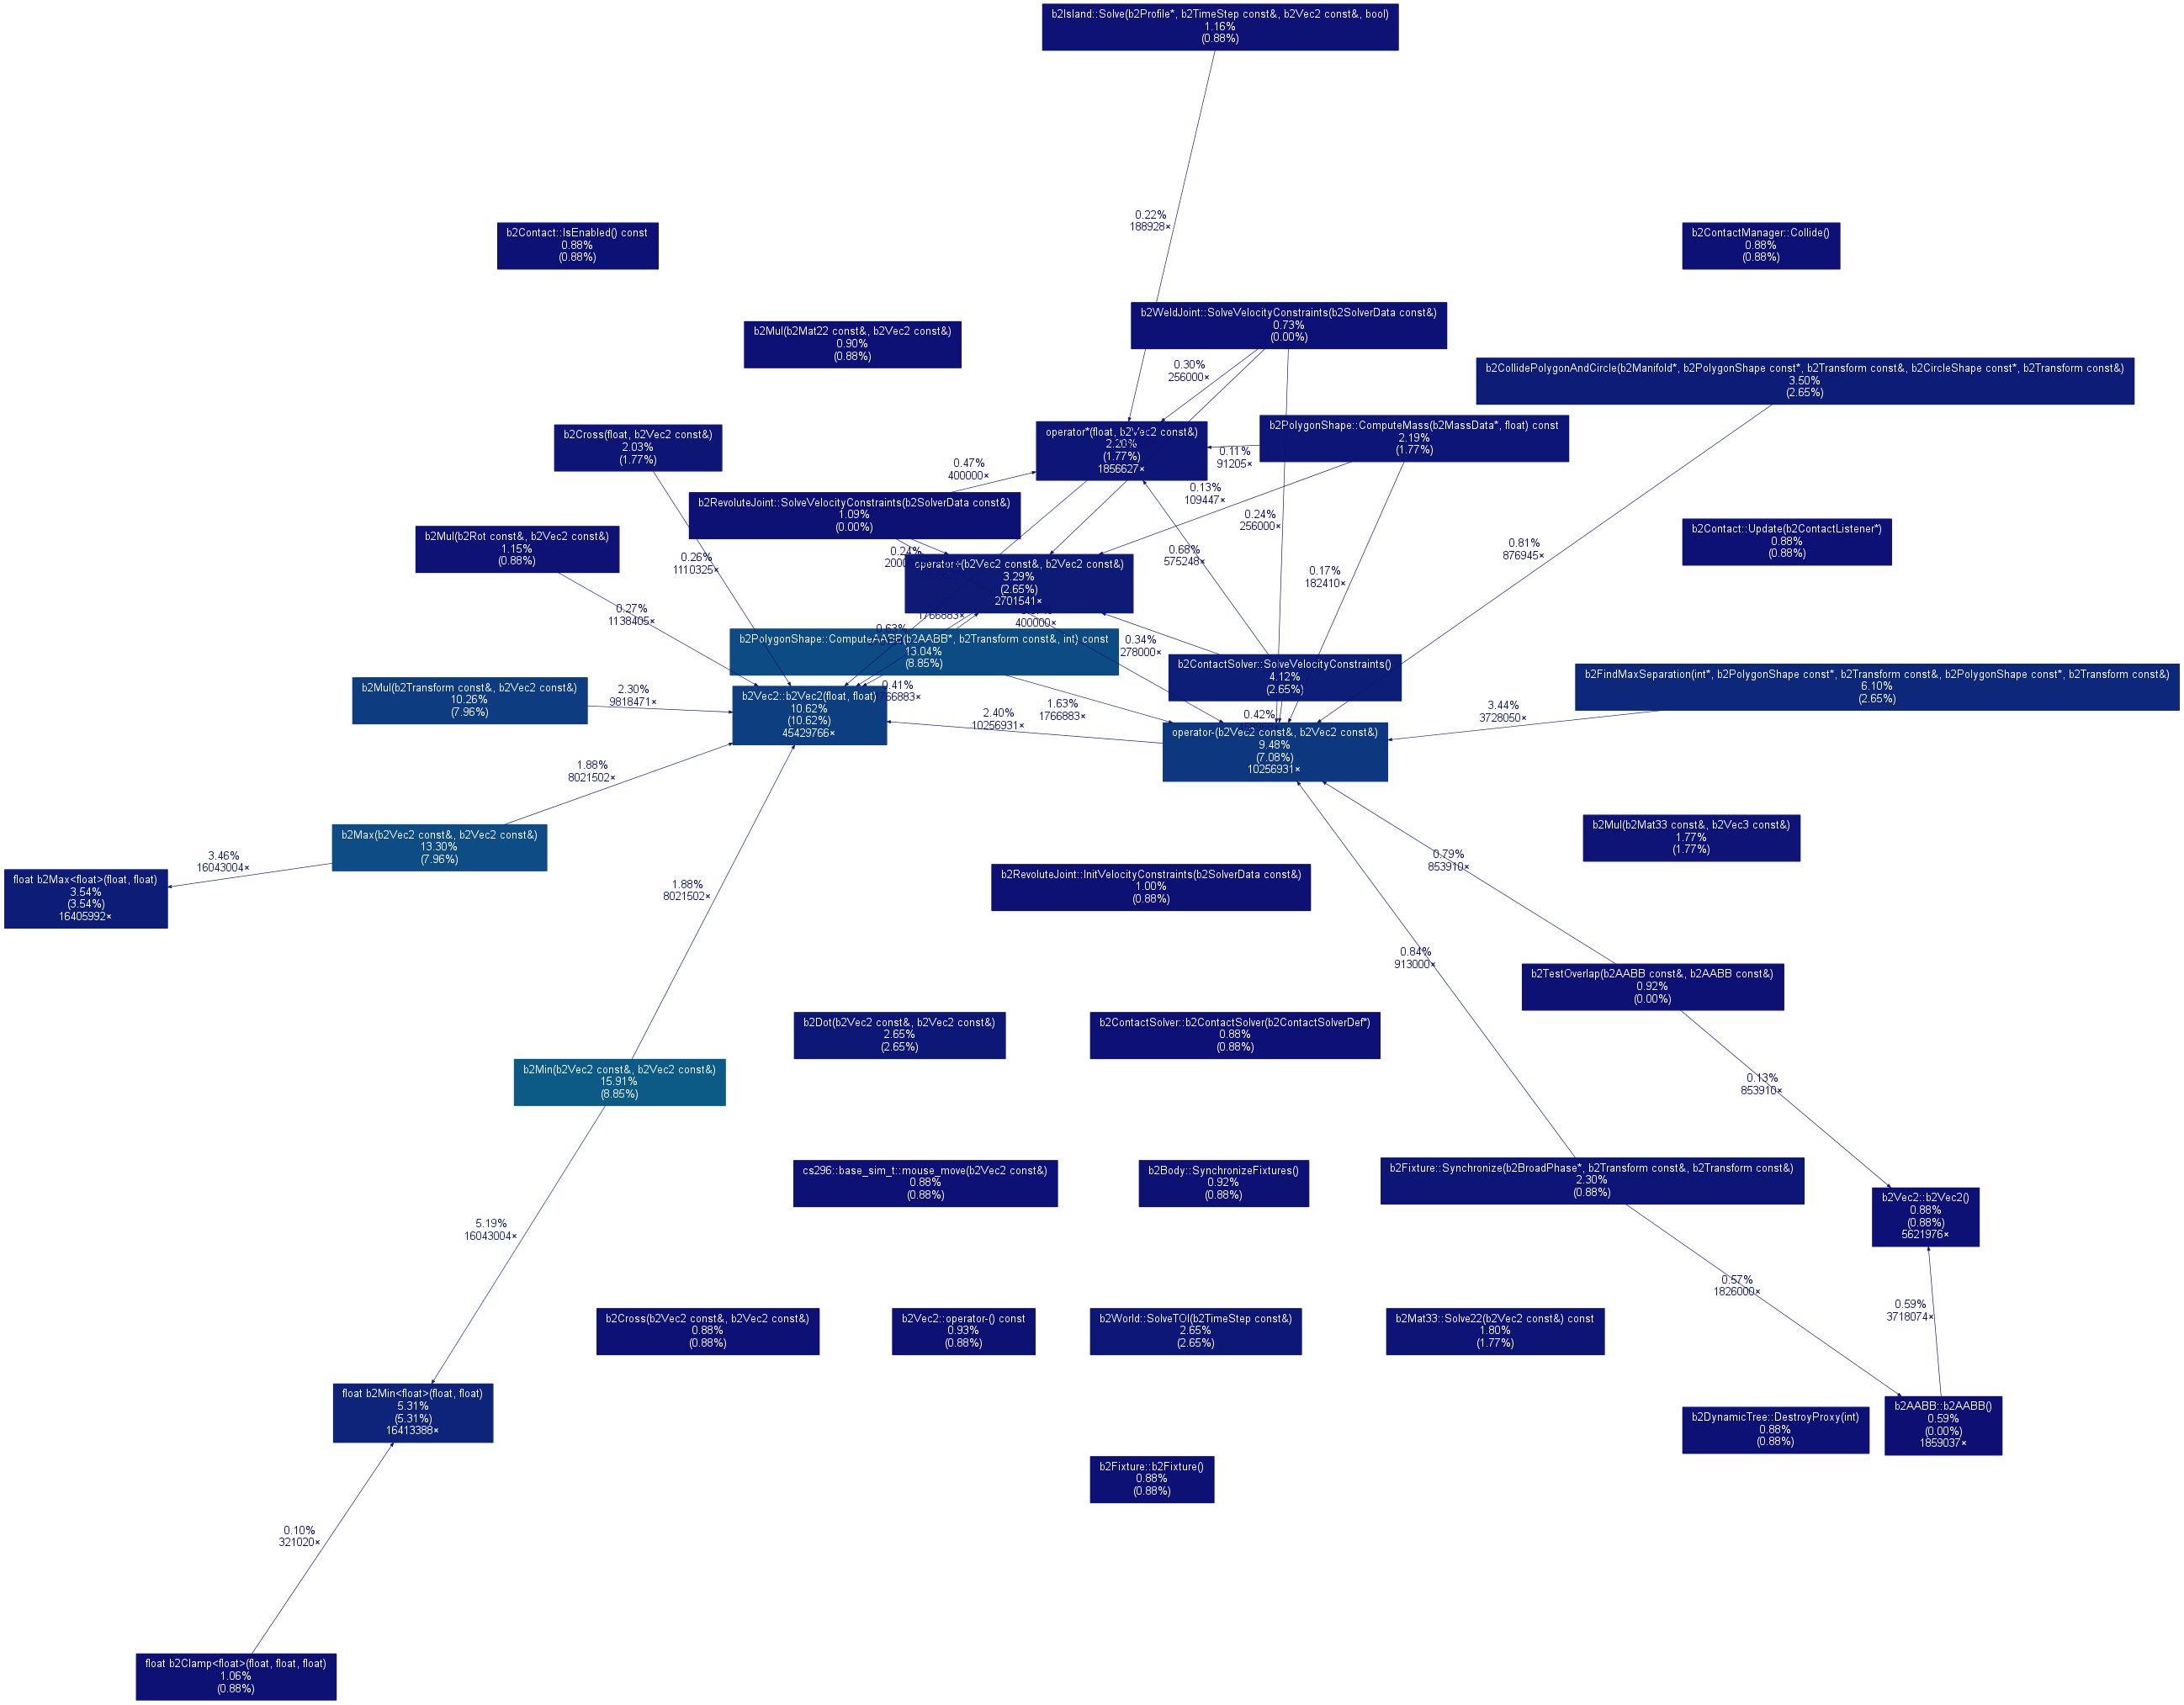
\includegraphics[scale=0.15]{./img/callgraph.png}
\\
As we can see, the b2Max b2Min, b2Mul, subtraction, and creation of vectors functions take up a lot of time. Combined,these took up nearly 50\% of the whole time. Hence these need to be highly optimised. On closer inspection, we see that the children function calls by these functions is significantly higher than their own self-times. 

Apart from these functions, we see that the operations (subtraction, multiplication etc.) take up significant time.   Another function that takes up a lot of time is the b2PolygonShape::ComputeAABB. A similar reason as above can be given for this.

Polygon colission takes very less time. This shows that box2d optimises polygon intersection routines and only checks it for the gear teeth which are close by. The high amount of time taken by ComputeAABB can be atributed to this fact that the number of polygons is huge, but this helps optimise colission routine, which is much heavier than calculating AABB of each fixture.

Our initial design had significantly higher number of objects than the current design. Hence, there, the time taken was more. So, when we minimised the number of gears and made the stack structure, we optimised our code. 

Further optimisation could have been possible if we would have used gear joints instead of manufacturing them ourselves, but that would have not looked as good as the current design and it would have been to easy to create. The current design is more consistent, robust and full of abstractions.


\subsection{Timing code}
Under heavy processor load, this is the graph we got.
\\
\\
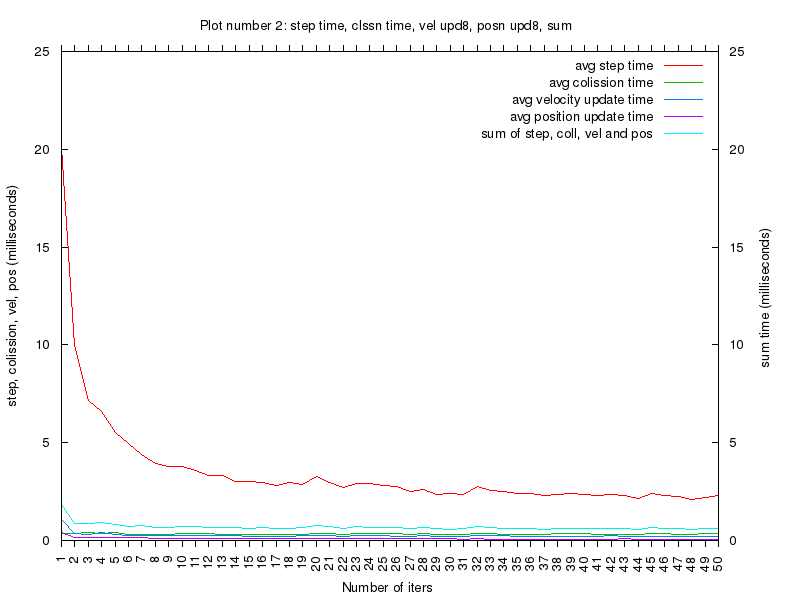
\includegraphics[scale=0.5]{./img/heavyload.png}
\\
Under light load, this is the graph we got.
\\
\\
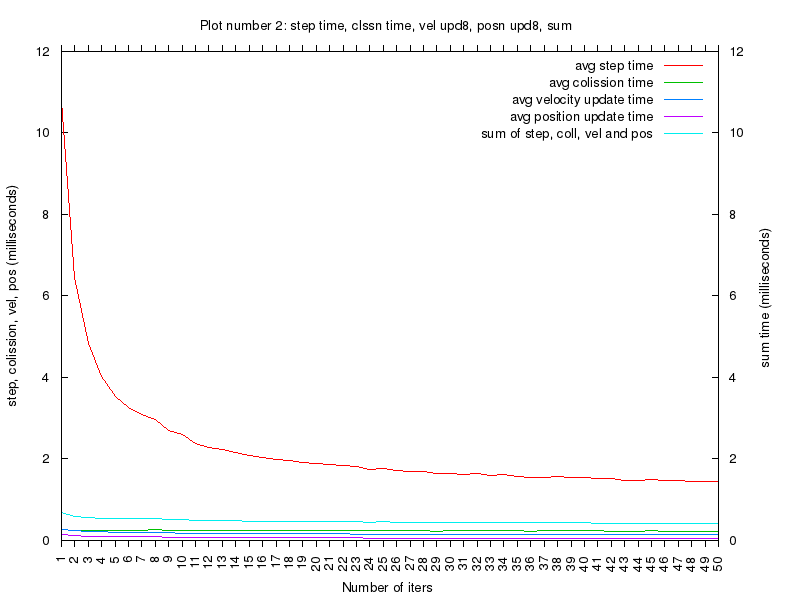
\includegraphics[scale=0.5]{./img/plot2.png}
\\ 

As we can see, the times have nearly doubled under heavy load.

\end{document}
}
